\documentclass[
    ngerman,american
    ]{scrartcl}

	% XeLaTeX
	% Biber
	
    % ##########################################
    % # Choose the language for the document by editing below line
    % # de = German
    % # en = English
    \newcommand{\lang}{en}
    % ##########################################
    \usepackage{babel}
    \usepackage[utf8]{inputenc} 
    \usepackage{csquotes}
    \usepackage{enumitem}
    \usepackage{ifthen}
    \usepackage{lipsum}
    \usepackage{graphicx}
    \usepackage{color}
    \usepackage{indentfirst}
    \usepackage{graphicx}
    \usepackage{float}
%   
\usepackage[colorlinks,linkcolor=blue]{hyperref}

    \setlength{\parindent}{2em}
    \include{translatedHeadings}
    
    \ifthenelse{\equal{en}{\lang}}
    {
        \selectlanguage{american} 
    }{
        \ifthenelse{\equal{de}{\lang}}
        {
            \selectlanguage{ngerman}
        }
        {\selectlanguage{american}}        
    }
\usepackage[
bibencoding=utf8, 
style=numeric,
sorting=none
]{biblatex}

\addbibresource{bibliography.bib}
%\bibliographystyle{unsrt}
% \bibliographystyle{unsrt} 
%    \usepackage[
%        bibencoding=utf8, 
%        style=numeric-comp,
%        sorting=none
%    ]{biblatex}

    \usepackage{amsmath}
    \title{
        % ##########################################
        % # Insert the title of your paper/thesis here
        % ###### 
        % Coming up with a good title is hard.
        % It should:
        %  1. capture the contents of the your work
        %  2. not be to broad or generic
        %  3. stick to the truth and don't not oversell
        %  4. use established terms and wordings
        %  5. make people curious about your work
        %  6. use current buzzwords if possilbe (but do it right)
        %  7. not use too many buzzwords :-)
        
        
        Overview of Past Projects Portfolio  
        % navigation / control 
        % ##########################################
        \\  \Large{\paperSubTitle{\lang}}} % don't touch this line
    \author{
        % ##########################################
        % # Your name goes here
        % ######
        % wWll, that should be obvious, right? 
      Xing-Yu Chen, M. Sc.
        % ##########################################
        }
  
\begin{document}  
%	\maketitle
%\tolerance=1
%\emergencystretch=\maxdimen
%\hyphenpenalty=10000
%\hbadness=10000

%\begin{abstract}
%% 腔道内介入手术机器人系统设计、手术导航、先进传感器与力反馈技术
%% 基于图像和数学融合模型的手术机器人智能控制方法
%% 该模型使用多模时间序列和空间信息数据集进行介入手术机器人的导航控制,并提高手术机器人的自主性
%% 动态数据+统计学习+临床验证
%% 应用人工智能提升特征参数识别率,创新柔性机器人器件微结构的设计方法
%% “自主制备传感/执行器件+多模力操控技能学习”的技术路线
%% 将传感器网络数据与术中图像等多模信息深度融合,提出了更有临场感的医生-手术机器人双向力反馈解决方案
%%传统的经自然腔道手术,只有视觉导航,现在要进行多模态信息的导航
%
%
%%            \ifthenelse{\equal{en}{\lang}}{}{}
%            % ##########################################
%Continuum robot has evolved as a novel treatment modality with better features over the traditional minimally invasive surgery, such as  faster, safer, and more convenient intra-body interventions without wide incisions. Several continuum surgical robot systems has been designed to navigate anatomical pathways through single-port access, e.g. natural orifice transluminal endoscopic surgery or minimal incisions. However, existing platforms lack intuitive navigation system due to limited and unreliable sources of feedback data. To address this issue and develop an improved continuum surgical robotic system with high safety-level, a novel intelligent navigation model is proposed based on multimodal data fusion. Investigations will be carried out towards developing a compact master-slave continuum robot platform that integrates multiple imaging modalities and sensors. Then, a robust fusion strategy will be developed for coupling multimodal information. Lastly, an intelligent navigation model will be proposed and developed with compliance control protocols.  
%
%
%Existing platforms currently underutilize the integration of motion, force, shape, and image data, lacking standardized methods for multimodal fusion-based navigation in continuum surgical robots. This proposal addresses two key scientific problems:
%i) investigating proximally and distally acquired motion, force, and shape data along with multiple imaging modalities to develop a standard multimodal data fusion method in real-time; and ii) modeling multimodal signals to develop reinforcement learning models with safe and efficient surgeon-robot compliance control. The successful implementation of this proposal is expected to provide an intelligent navigation system with compliance control protocols that seamlessly support surgeon-robot collaboration, thereby improving the current treatment modality.  
%
%
%
%\end{abstract}
%\sectionBackground{\lang}
%\sectionBackgroundDescription{\lang}



\maketitle
\sectionQuestions{\lang}
%\sectionQuestionsDescription{\lang}
        
Continuum robot has evolved as a novel treatment modality with better features over the traditional minimally invasive surgery, such as faster, safer, and more convenient intra-body interventions without wide incisions. They are designed to navigate
anatomical pathways through single-port access, e.g. natural orifice transluminal endoscopic surgery or minimal incisions. Continuum surgical robots have a fundamentally different structure than
conventional manipulators composed of discrete rigid links connected by joints. Their
ability to take the shape of 3D curves enables these robots to perform procedures
through smaller surgical corridors than would be possible with traditional robotic
mechanisms.
During the work in Shenzhen Institute of Advanced Technology, Chinese Academy of Sciences, I lead a small group of students and design two continuum robot, a vascular interventional surgical robot and a robotic bronchoscopy system.


\subsection{Novel Robotic Bronchoscopy System}


Related Pubulication: 

\textbf{Chen, Xing-Yu}, et al. \href{https://doi.org/10.13140/RG.2.2.24714.64963}{\textit{Design of a Teleoperated Robotic Bronchoscopy System for Peripheral Pulmonary Lesion Biopsy.}}  \textit{arXiv preprint arXiv:2306.09598}(2023).



CN Patent: \emph{\href{https://www.researchgate.net/publication/370801235_CN_Patent_yizhonggangdulianxukediaoqiaoguanjiqigangdudiaojiefangfaheshoushushebei}{A sheath with continuously adjustable stiffness, its stiffness adjustment method, and surgical equipment.}} CN115920200A.

CN Patent: \emph{\href{https://www.researchgate.net/publication/370801423_CN_Patent_yizhonghuojianqianshounayudisongzhuangzhiyijizhiqiguanjingshoushujiqiren}{Biopsy Forceps Storage and Delivery Device for Bronchoscope Surgical Robots.}} CN115429343A.


CN Patent: \emph{\href{https://www.researchgate.net/publication/370801247_CN_Patent_yizhongjinghuxidaozhenliaojiqirenxitongjiqikongzhifangfa}{A Respiratory Diagnosis and Treatment Robot System and its Control Method.}} PCT/CN115252146.


CN Patent: \emph{\href{https://www.researchgate.net/publication/372234328_CN_Patent_yizhongzhiqiguanjingmozujiqihuojianfangfahecaiyongqideshoushujiqiren}{A bronchoscope module and its biopsy method.}}  CN116369834A.
~\\

I am currently tasked with designing an innovative teleoperated robotic bronchoscopy system and multi-modal navigation through image and electromagnetic sensors. During the procedure, the surgeon holds a tablet console to control a flexible visual bronchoscope, inserts a flexible tube into the patient's mouth, and utilizes the robot for advancements, rotations, and adjustment of the bending angle of the front end of the flexible bronchoscope. The robot also enables control of the biopsy forceps for feeding and tissue sampling. 

\begin{figure}[H]
	\centering{\includegraphics[width=0.8\columnwidth]{fotos/R_B_system.pdf}}
	\caption{Robotic Bronchoscopy System. (A) Robot and bronchus phantom; (B) Biopsy forceps manipulator; (C) Bronchoscopic video. (D) EM-Sensor based navigation system; (E) Embedded control system, electrical devices and motors; (F) Biopsy forceps and Catheters delivery device.}
	\label{RBSystem}
\end{figure}



\begin{figure}[H]
	\centering{\includegraphics[width=0.7\columnwidth,height=0.4\columnwidth]{fotos/structure.pdf}}
	\caption{Structure of the bronchoscope robot.}
	\label{structure}
\end{figure}

The system consists of a teleoperated surgical robot designed for trans-respiratory diagnosis, along with a corresponding master-slave control system. It incorporates various components, including a flexible bronchoscope, bronchial biopsy instruments, variable stiffness catheters, a magnetic navigation device, and several tablets functioning as master consoles. The surgeon operates the tablet, and the instructions are wirelessly transmitted to the embedded system controller through the TCP/IP protocol suite. Subsequently, the robot manipulates the flexible bronchoscope in response to the issued commands. Employing a multi-operator strategy, the robot is controlled through scheduling arrangement and weight distribution, which enables mentor surgeons and trainee surgeons operate surgery simultaneously. They can observe the same surgical site and share control of robotically controlled surgical instruments. This allows trainees to gain firsthand experience of the procedure while being guided by the mentor surgeon. Additionally, the mentor surgeon can switch control to selected trainees if necessary and override their control during the bronchoscopy procedure. I developed the electrical system of the entire surgical robot, and used pyqt to design the UI interface of the system, as shown in Fig.\ref{three_tools}. We have also developed a novel Variable Stiffness Catheter (VS-Catheter) composed of Low Melting Point Alloy (LMPA) to enhance the catheter's flexibility in the context of minimally invasive surgery and expand the accessible area for bronchoscopic biopsy forceps. Compared with bronchoscope, the VS-Catheter can be inserted into narrower bronchi and offers more flexible control with dynamic stiffness.   

\begin{figure}[H]
	\centering{\includegraphics[width=0.95\columnwidth,height=0.45\columnwidth]{fotos/architecture.pdf}}
	\caption{Proposed three-stage bronchoscopy surgical procedures, with initial insertion, dynamic adjustment, and tissue sampling.}
	\label{three_stage}
\end{figure}


\begin{figure}[H]
	\centering{\includegraphics[width=0.8\columnwidth,height=0.55\columnwidth]{fotos/model_the_three3.pdf}}
	\caption{(A) Proposed robotic bronchoscopy system. (B) UI developed with PyQt. (C) Novel three-stage bronchoscopy surgical procedure composed of robotic bronchoscope, VS-Catheter, and tissue sampling by biopsy forceps. (D) The three-stage bronchoscopy surgical tools.}
	\label{three_tools}
\end{figure}


Additionally, to integrate endoscopic video and EM tracking information, I am employing a multimodal navigation system, utilizing the open-source software 3D Slicer, shown in Fig.\ref{3dsclicer}. It offers a range of tools for importing, processing, visualizing, and analyzing medical image data. It also provides capabilities for image registration, segmentation, and fusion. Furthermore, it includes a toolbox of navigation features, image-processing algorithms, and connections to external hardware for image-guided therapy (IGT). By combining images, tracked surgical instruments, and computer display, a comprehensive navigation system is created, enabling real-time identification of the direction and position of the bronchoscope tip and reference.


\begin{figure}[H]
	\centering{\includegraphics[width=0.7\columnwidth,height=0.4\columnwidth]{fotos/3dslicer.jpg}}
	\caption{3D Slicer and coordinate transform.}
	\label{3dsclicer}
\end{figure}

Fig.\ref{Procedure} showed the surgery procedure of robot-assisted bronchoscopy. Registration involves creating a 3D map of the patient's airways, integrated through CT or MRI to provide visual map of the surgical workspace. This map is used to guide the robotic system during the procedure. Once the registration is complete, the physician will use the 3D map to plan the bronchoscopy procedure. This may involve identifying the location of suspicious areas, such as tumors or lesions, and planning the best route to reach them. After the robotic system is set up on a passive arm and calibrated, the physician remotely controls the robotic system to examine the patient's airways with virtual bronchial navigation or EM guidance  navigation system, looks for any abnormalities or suspicious areas, and performs a biopsy or other procedure to obtain a tissue sample for further testing.	




\begin{figure}[H]
	\centering{\includegraphics[width=1\columnwidth,height=0.45\columnwidth]{fotos/navigation_procedure.pdf}} 
	\caption{Robotic assisted bronchoscopy procedure.}
	\label{Procedure}
\end{figure}      

\begin{figure}[H]
	\centering{\includegraphics[width=0.7\columnwidth]{fotos/experiment.pdf}}
	\caption{Proposed bronchoscopy system. (A) In-vivo experiment; (B) The	three-stage bronchoscopy tools in pig’s trachea.}
	\label{animal}
\end{figure}

In addition, we conducted several animal biopsy experiments using the robotic bronchoscopy system, as depicted in Fig.\ref{animal}. The system was controlled by two operators using tablets with different priorities and EM sensors were attached to the pig's forebreast and the tip of the bronchoscope. We successfully performed a biopsy procedure in which small tissue was clamped and removed from the tertiary bronchus of a pig. The implementation of the VS-Catheter enabled more flexible control of the biopsy forceps within the bronchus. The stiffness of the catheter was adjusted by energizing the resistance wire, providing adaptability based on the specific requirements of the procedure. The usability and effectiveness of the designed bronchoscopy surgical robot were demonstrated. Our work has been submitted to the 2023 IEEE BioCAS conference for publication.








	\subsection{Vascular Interventional Surgical Robot}
Related pubulication: 	

\textbf{Chen, Xing-Yu}, et al. \href{https://doi.org/10.3390/fib10120106}{\textit{Design and Evaluation of a Learning-based Vascular Interventional Surgery Robot.}} \textit{Fibers}, 10.12 (2022): 106.

Akinyemi, T.O., et al.   \emph{\href{https://doi.org/10.3390/app122110936}{ Adapting Neural-Based Models for Position Error Compensation in Robotic Catheter Systems.}} \textit {Applied Sciences}, 12.21 (2022): 10936.

Akinyemi, T.O., et al.   \emph{\href{https://doi.org/10.1109/JSEN.2023.3281009}{Interventionalist Hand Motion Recognition with Convolutional Neural Network in Robot-assisted Coronary Interventions.}} \textit{IEEE Sensors Journal}.

Duan, Wenke, et al. \emph{\href{https://doi.org/10.3390/mi14010197}{Technical and Clinical Progress on Robot-Assisted Endovascular Interventions: A Review.}} \textit{Micromachines}, 14.1 (2023): 197.

CN Patent: \emph{\href{https://www.researchgate.net/publication/370801433_CN_Patent_yizhongshoushujiqirendezhuduanliganzhifankuicaozongzhuangzhijifangfa}{A Tactile-Feedback Device and Method for Surgical Robots.}} CN115137483A.


CN Patent: \emph{\href{https://www.researchgate.net/publication/370801270_CN_Patent_yizhongshuangxiangdianchushijierujiqirencongduandaosilijiancezhuangzhijifangfa}{ A Bidirectional Guidewire Force Measurement Method for Vascular Interventional Surgical Robot.}} CN114948258A.
~\\	

I have designed an isomorphic master-salve Vascular Interventional Surgical Robot (VISR) for precise force measurement and navigation of endovascular tools viz. catheters and guidewires, as shown in Fig.\ref{VISR}-\ref{architecture1}. The master console aids operators in issuing manipulation commands and logs feedback from the force, rotation, and translation data. The slave manipulator uses the commands received from the master platform for actual tool navigation. Some force sensors are mounted at clamping device of the robot manipulator, so I utilized an Artificial Neural Network (ANN) for guidewire resistance force modulation with 50 mN precision. The developed ANN is a multilayer perceptron with five hidden layers and 77 neurons. The network is used to estimate distal force of guidewire from the force measured from force sensor in robot manipulator. 

\begin{figure}[H]
	\centering{\includegraphics[width=0.8\columnwidth,height=0.6\columnwidth]{fotos/VISR.png}}
	\caption{Vascular interventional surgical robot designed in SIAT, Chinese Academy of Sciences; (A) Master console; (B) Slave manipulator; (C) Surgeons teleoperate the master console in the room without being exposed to X-rays; (D) Slave manipulator placed next to pig in DSA room.}
	\label{VISR}
\end{figure}   


\begin{figure}[H]
	\centering{\includegraphics[width=0.8\columnwidth]{fotos/control_flow.pdf}}
	\caption{Control flow of the VISR. Surgeons teleoperate the doctor’s terminal in the room without
		X-rays, and the slave manipulator with a robotic arm is placed beside the patient’s bed.}
	\label{control_flow}
\end{figure}


\begin{figure}[H]
	\centering{\includegraphics[width=0.8\columnwidth]{fotos/architecture1.pdf}}
	\caption{Layers of the VISR control architecture.}
	\label{architecture1}
\end{figure}


As shown in Fig.\ref{forcebox}, the robotic system includes a force box used for measuring the
tactile force that interventionalists exerted with their fingers. This force is regarded as the
interventionalists’ operative force on the guidewire or catheter in regular surgery. The force box includes a 32-prism, tiny flexible strip sensors, PCBs, and batteries. A flexible
sensor is folded and wound around the force box surface, and its data is logged as a
32-channel data multiplexed over an Analog Multiplexer (Texas Instruments). Thus, the interventionalists also operate the master device by manipulating the
flexible sensor with their finger. The force data is processed in a microcontroller STM32
 and transmitted over a Bluetooth module to the slave console in real time. The force box also reflects
information about the flexible tool’s firmness as it is held with a clamping mechanism in
the slave manipulator. The guidewire is clamped tightly when the surgeon presses hard on
the force box and vice versa.

\begin{figure}[H]
	\centering{\includegraphics[width=0.8\columnwidth,height=0.3\columnwidth]{fotos/forcebox.pdf}}
	\caption{The structure of the force box, which can measure the tactile force exerted by the surgeon's fingers. The force value will be used as parts of multi-modal information to optimize the control algorithm. (A) PCB layout of force box; (B) Force box includes a 32-prism,  tiny flexible strip sensors. }
	\label{forcebox}
\end{figure}   


To study the usage of robotic-assisted vascular interventions by surgeons and aid them in acquiring skills more efficiently, I designed a smart glove shown in Fig.\ref{glove}. This glove is capable of capturing and fusing information from multiple modalities, including the bending of the surgeon's fingers, the forces exerted while manipulating the vascular surgical robot, electromyographic (EMG) signals, posture angles and accelerations (IMU), as well as spatial position and orientation collected using electromagnetic sensors.


\begin{figure}[H]
	\centering{\includegraphics[width=0.8\columnwidth,height=0.55\columnwidth]{fotos/glove.pdf}}
	\caption{Intelligent glove for robotic catheterization skill learning. }
	\label{glove}
\end{figure}   


In addition, I utilized fuzzy PID and recurrent neural network (RNN) models such as the Long Short-Term Memory networks (LSTM) and Gated Recurrent Unit (GRU) networks to learn typical motion dynamics when running the master-slave platform. The trained network could estimate the position of the slave robot based on input motion factors. The estimated value and an appropriate compensatory value are then transferred to the slave robotic device in order to map the master platform's movements uniformly.     
The RNN models were implemented in Python and using the Keras library and the TensorFlow framework. The LSTM model contains an input layer (N$\times$3$\times$3), two hidden layer with 32 units each, and a fully connected layer that outputs a predicted value using the rectified linear unit (ReLU) activation function. The LSTM unit may extract essential features from an input sequence and store them in memory. To train the model, experimental data for various step values was stacked together, and feature scaling was applied to the data. 


\begin{figure}[H]
	\centering{\includegraphics[width=0.8\columnwidth,height=0.3\columnwidth]{fotos/position_prediction.png}} 
	\caption{A stacked 2-layer architecture for robot position prediction and compensation using (a) LSTM and (b) GRU model.}
	\label{LSTM_GRU}
\end{figure}   
%
\begin{figure}[H]
	
	\centering{\includegraphics[width=0.72\columnwidth,height=0.18\columnwidth]{fotos/control_block.png}} 
	\caption{Control block with error compensation for the patient-side robot.}
	\label{control_block}
\end{figure}   

Fig.\ref{LSTM_GRU} depicts the in-silico evaluations of the GRU and LSTM-based controllers. Although the original error increased to 40\%(2.0mm) of the input command for several phases, the minimum and greatest final errors were 0.001 mm and 0.1mm (2\% of the input command) across the steps. It depicts how the GRU-based controller may estimate the predicted slave robot response ahead of time and then use this to regress the initial position error. To validate the real-time usability of the learning-based models in the VISR, we utilized the Jetson AGX Orin development kit (NVIDIA, CA, USA) for the patient-side robot, and evaluated the model's performance under uniform and varying input commands using the control block diagram presented in Fig.\ref{control_block}. For a typical master's displacement, velocity, and the velocity ratio, the RNN model makes an appropriate prediction and checks for errors.  

	
	
	
%The idea of this proposal is based on integrating multi-modal data from motion, force, position and image information to develop an intelligent navigation strategy for safe and efficient robotic surgery. The research contents are given as follows: 
%
%1) development of a compact master-slave continuum robot platform for precise and safe surgery navigation, with sub-millimeter precision resolution for linear, rotary, and hybrid tool movements. 
%
%2) designing efficient methods for real-time modeling and compensation of hysteresis in the continuum robot when driven with underactuated robotic systems. This will include analysis of force hysteresis curve of continuum robot between proximal and distal force sensor, and development of a novel motion compensation framework with machine learning-based control algorithm.
%
%3) modeling information fusion strategy for real-time coupling of proximally and distally acquired motion, force, shape and image data. This will include integration of optical or electromagnetic tracking and other sensing devices with surgical instruments, and the development of cross-modal data fusion for compliant robot-assisted surgery. 
%
%4) establishing a high-fidelity robotic surgery force and visual feedback technique based on theoretical analysis and simulation modeling for intelligent navigation using the coupled multimodal data. 
%  
%5) development of novel reinforcement learning-based strategy with robot navigation towards safe surgeon-robot interaction and task autonomy. This is envisioned by utilizing feedback control systems through intraoperative multimodal imaging and sensor data fusion to guide a surgical procedure.
%    
    
    

\section{Driver Board of 4D Ultrasound}


The 4D imaging in sonography is an advanced technique that enables real-time 3D ultrasound imaging of the fetus within the body, incorporating the element of time or motion. This technique is commonly employed in obstetrics to assess fetal growth, development, and identify any potential abnormalities or malformations. Furthermore, it finds application in various medical contexts, such as visualizing the heart or blood vessels in real-time. The introduction of 4D imaging has revolutionized prenatal imaging, granting expectant parents the opportunity to observe detailed, dynamic images of their developing baby in the womb.

During my previous work at Esaote, one of the world's leading ultrasound manufacturers, I actively contributed to the design of a novel ultrasound scanner system, as depicted in Fig.\ref{4DPCB}. This experience provided me with a comprehensive understanding of the underlying principles and implementation methods of ultrasonography. The TMC5130A (Trinamic, Hamburg, Germany) served as a high-voltage general-purpose controller for two-phase bipolar stepping motors. Notably, this chip featured a serial communication interface, enabling automated target positioning. When paired with an external power transistor, it facilitated high dynamic range and high torque motor control.

The central function of the 4D driver board's CPU was to receive data from the host motherboard and issue various motor control instructions to the TMC5130A. To fulfill this role, I utilized the STM32F3 series chip, a 32-bit MCU based on ARM's Cortex-M4 core. With a voltage supply range of 2.0 to 3.6V, this microcontroller boasted 16k bytes of SRAM, two SPI interfaces, one ADC, and three USARTs. It supported crystal oscillators ranging from 4 to 32MHz and offered debugging capabilities via SWD or JTAG, effectively catering to the requirements of the 4D driver board's main control chip. The communication between the motor driver TMC5130A and the microcontroller STM32 was established using the SPI protocol.




\begin{figure}[H]
	
	\centering{\includegraphics[width=0.95\columnwidth,height=0.57\columnwidth]{fotos/4DProbe.pdf}}
	\caption{4D probe system. (A) Structure of 4D probe; (B) 4D probe driver; (C) PCB layouts; (D) 4D probe driver in the ultrasound system, the PCB is inserted into the motherboard.}
	\label{4DPCB}
\end{figure}  


To mitigate the interference caused by the drive signal from the motor driver in the 4D-Probe, which affected the received signal from the ultrasonic transducer and introduced noise in the 4D imaging, I undertook several optimization measures. Firstly, I focused on optimizing the PCB layout of the motor driver within the 4D-Probe. By carefully arranging the components and traces, I aimed to minimize signal coupling and electromagnetic interference. Furthermore, I implemented shielding covers to establish spatial isolation for the motor driver. These covers acted as a barrier, preventing the drive signal from directly affecting the sensitive components and circuitry involved in receiving the ultrasonic signals. This shielding approach effectively reduced unwanted noise and interference. In addition, I incorporated layered ground structures into the design to counteract any interference stemming from ground currents. This involved creating separate ground planes and carefully managing the routing of ground connections, which aided in minimizing signal crosstalk and further enhancing the overall performance of the ultrasound imaging system. By implementing these optimization techniques, I successfully addressed the issue of signal interference and crosstalk, leading to improved image quality and enhanced signal integrity in the 4D imaging process, as shown in Fig.\ref{4D}.   



\begin{figure}[H]
	
	\centering{\includegraphics[width=0.6\columnwidth,height=0.4\columnwidth]{fotos/4D.png}}
	\caption{4D imaging in sonography. (A) Fetal ultrasound training phantom; (B) Noise in the 4D imaging system; (C) Signal crosstalk eliminated; (D) Reconstructed fetus model.}
	\label{4D}
\end{figure}  







\section{Magnetic Nanoparticle Imaing Scanner}


 As an emerging tomographic imaging modality, Magnetic Particle Imaging (MPI) has many
 potential uses in biomedical engineering. It measures the magnetization response of superparamagnetic
 iron oxide nanoparticles and images the spatial distribution of tracer material.
 Unlike other tomographic imaging techniques, such as Positron Emission Tomography (PET)
 and Single Photon Emission Computed Tomography (SPECT), MPI is entirely free of
 ionizing radiation, which benefits the safety of patients and medical staff.
 The main challenge faced by many researchers is the detection sensitivity of the MPI scanner
 and the high signal-to-noise ratio (SNR) requirements in the MPI system. The amplitude of
 the signal, which is detected by the receive coil, could be extremely low. In this situation,
 the signal must be amplified with a low-noise amplifier (LNA). In master's thesis at TU Braunschweig, I focused on analyzing the noise characteristics of the MPI receive system and proposed two methods to improve the noise performance over a wide-band frequency range: a ferrite core transformer and a LNA. The prototype LNA consisted of four parallel amplifiers and a summing circuit, resulting in a significant improvement in the noise performance of the MPI receive chain.
 
  \begin{figure}[H]
 	\centering{\includegraphics[width=0.95\columnwidth,height=0.35\columnwidth]{fotos/MPI_model.pdf}}
 	\caption{Principle of Magnetic Particle Imaging. (A) The relationship between the external magnetic field and the magnetization of magnetic nanoparticles. (B) Noise model of the MPI scanner receive chain. }
 	\label{MPI_model}
 \end{figure}  
 
 \begin{figure}[H]
 	
 	\centering{\includegraphics[width=0.8\columnwidth,height=0.36\columnwidth]{fotos/MPI.pdf}}
 	\caption{Magnetic Particle Imaging system in TU Braunschweig, Germany. (A) MPI scanner. (B) Proposed LNA and  ferrite core transformer. }
 	\label{MPI}
 \end{figure}  
 
%     
%\section{Electromagnetic Metamaterials and Antennas }     
%Related Pubulication: 
%
%Liu, Liangliang, et al. \emph{\href{https://doi.org/10.1063/1.4907879}{High-efficiency transition between rectangular waveguide and domino plasmonic waveguide.}} \textit{AIP Advances}, 5.2(2015), 027105.
%  
%CN Patent: \emph{\href{https://cprs.patentstar.com.cn/Search/Detail?ANE=9DEA3ADA9EIE9AHC6DCA6BFA9HAA6AGA9HBFCHFA9EGG9ADB}{A rectangular waveguide to domino plasmonic waveguide converter.}} CN103985942B.
% 
% CN Patent: \emph{\href{https://cprs.patentstar.com.cn/Search/Detail?ANE=9BHB9CHA9IDD9BFB9DFA9HIG7EBA6AGA9CFF9GFCBIIA9EGF}{A coaxial waveguide to artificial surface plasmon waveguide converter.}} CN103985944B.
%
%\subsection{Electromagnetic Band Gap}
%
%
%
%Electromagnetic Band Gap (EBG) structure is a kind of metamaterial, the utilization of EBG is
%becoming attractive in the antenna community in recently years. EBG structures can greatly
%improve performance of Antenna, limitations of designs of traditional antennas are broken, which
%would bring huge changes and improvements for antennas in wireless communication systems.
%Therefore, it has very high academic value and application value to do research on EBG
%structures and its applications in antennas for enhancing the efficiency. In my bachelor thesis, I designed several EBG metamaterial structures to improve antennas' work efficiency and several FBG structures with an antenna reflector substrate, simulated them using software CST. Fig.\ref{EBG} - \ref{Waveguide} show one example of designed EBG structure for dual band microstrip antenna.
%
%
%
%
%\begin{figure}[H]
%	\centering{\includegraphics[width=0.7\columnwidth,height=0.30\columnwidth]{fotos/EBG.pdf}}
%	\caption{(A) Dual-frequency antenna with a circle of dual-frequency UC-EBG structure; (B) Reflection coefficient.}
%	\label{EBG}
%\end{figure}  
%
%
%
%
%\begin{figure}[H]
%	\centering
%	\begin{minipage}[t]{0.45\textwidth}
%		\centering
%		\includegraphics[width=0.75\columnwidth,height=0.7\columnwidth]{fotos/EBG_Simulation.pdf}
%		\caption{Microstrip antenna field diagram before and after loading dual-band EBG. (A) 4.5GHz before; (B) 4.5GHz after; (C) 7.4GHz before; (D) 7.4GHz after.}
%	\end{minipage}
%	\begin{minipage}[t]{0.45\textwidth}
%		\centering
%		\includegraphics[width=0.9\columnwidth,height=0.75\columnwidth]{fotos/EBG_Chart.pdf}
%		\caption{Radiation Pattern. (A) H-plane in 4.5 GHz; (B) E-plane in 4.5 GHz; (C) H-plane in 7.4 GHz; (D) E-plane in 7.4 GHz.}
%	\end{minipage}
%\label{simu}
%\end{figure}
%
%
%
%\subsection{Domino Plasmonic Waveguide}
%
%During undergraduate years, I joined the Key Laboratory of Radar Imaging and Microwave Photonics, the Ministry of Education, China. We proposed an optimized transition structure to realize smooth and high
%efficiency conversion from the guided wave supported by a conventional rectangular waveguide (CRW) to the domino plasmon polaritons (DPPs) supported by a domino plasmonic waveguide (DPW) and vice versa in the X-band (8.2GHz∼12.4GHz). This transition structure consists of two tapered CRWs connected by a gradient domino array with optimized gradient heights and lateral widths. Experimental
%results of the S-parameters show excellent agreement with the simulations and
%the optimization scheme can be readily extended to other bands. Furthermore, a
%domino plasmonic power divider is implemented to demonstrate the application of
%the transition structure in the integration of conventional microwave circuits with
%plasmonic devices.
%
%
%
%\begin{figure}[h]
%	\centering{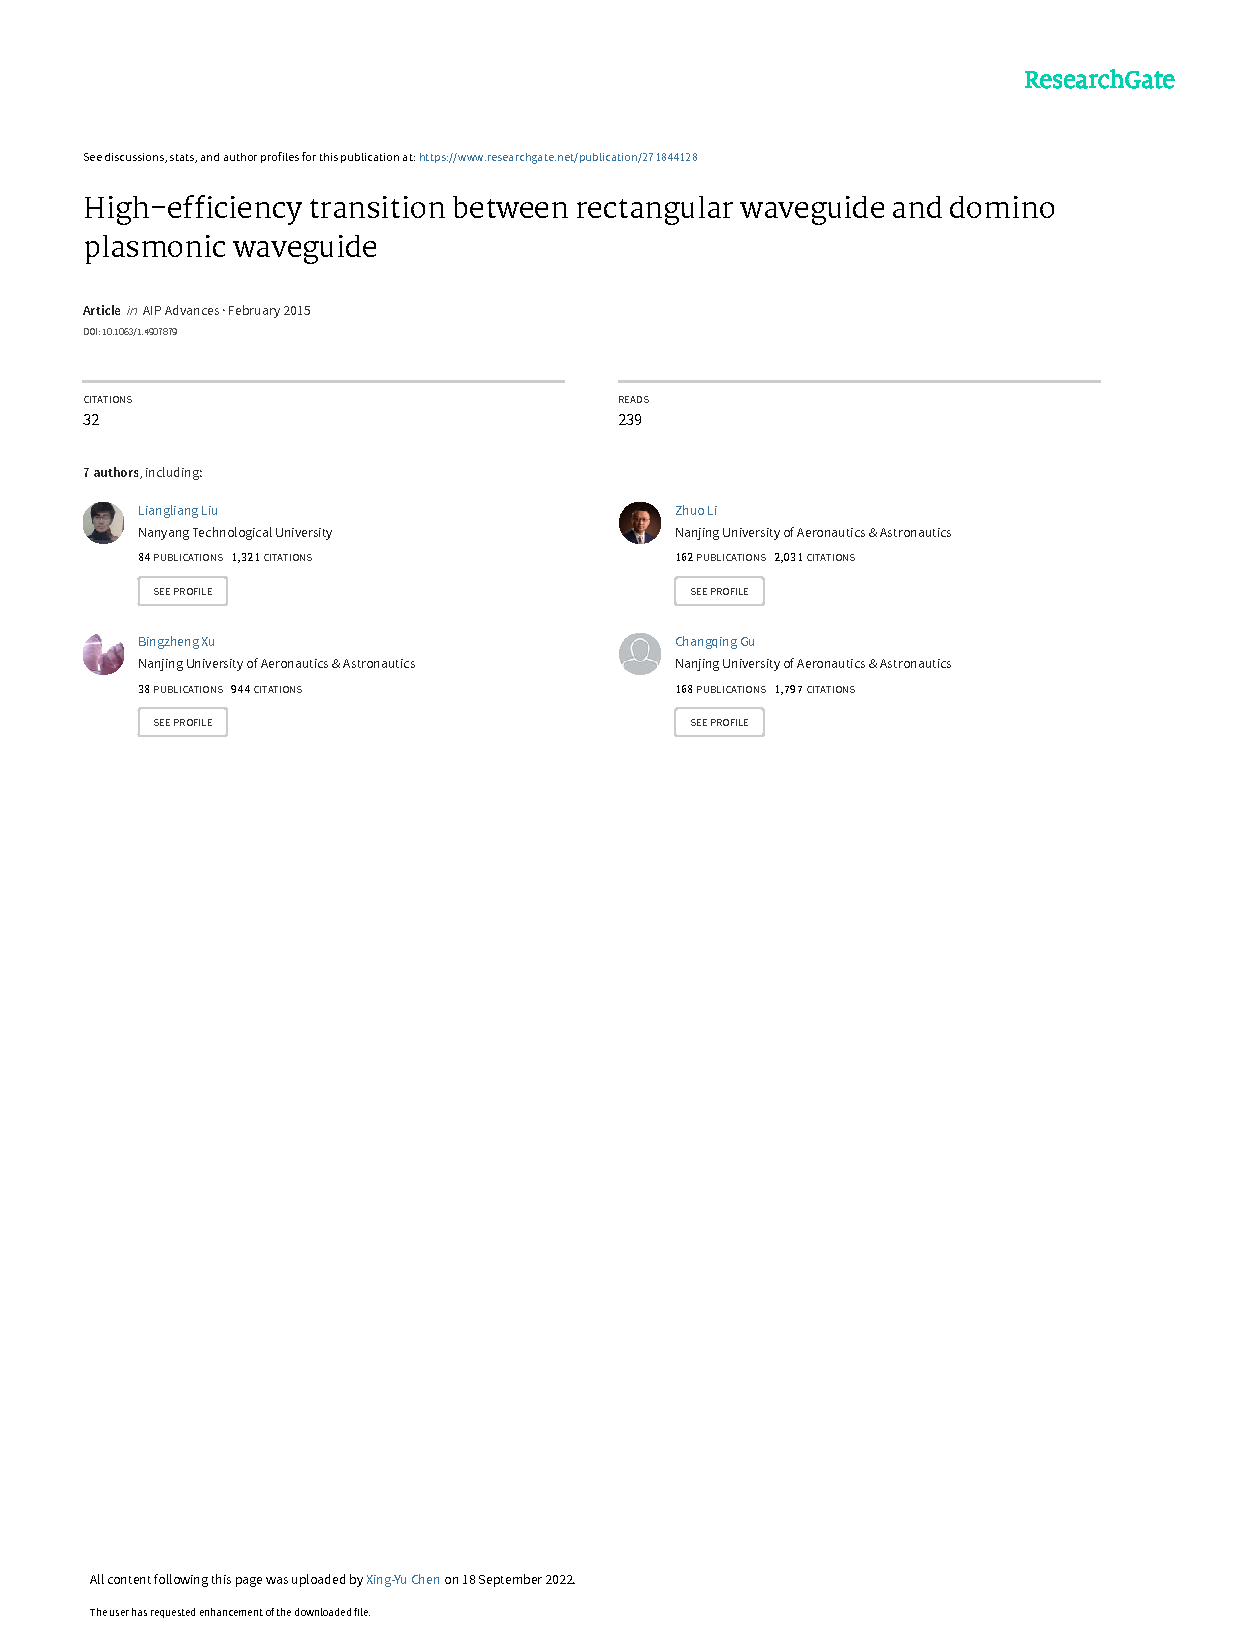
\includegraphics[width=0.7\columnwidth,height=0.26\columnwidth]{fotos/waveguide.pdf}}
%	\caption{Domino	plasmonic waveguide. (A) The Setup for the S-parameters measurement; (B) The simulated and measured S-parameters of the proposed tructure with the matching transition.}
%	\label{Waveguide}
%\end{figure}  
%





    \clearpage    
    

%\bibliography{bibliography}
\end{document}